\chapter{The Workhorses of Electronic Structure Theory}
\label{chap:gw}
\noindent
\section{Introduction}
In this chapter we discuss the theory underlying the 
the $GW$ approximation to obtain a quantitative {\it ab initio} 
description of electronic excitations. Density functional theory
is also discussed because it provides a useful starting point for
performing $GW$ calculations. The guiding principle for treating electron 
correlation followed here is to start from the "best possible" ground state description
that can be calculated precisely. This may be a Hartree-Fock ground state,
a DFT ground state, a ground state computed using some mixture of exact exchange
and DFT etc. While the Green's function formalism allows for systematic
inclusion of higher and higher order interactions in keeping with the "materials
science as a craft" approach it is much more efficient to start from the most 
favourable position possible: i.e., the best single particle description we can obtain.

To make the connection with the tight-binding recursion method 
we need to transform our ground state (however it might be obtained), into a
Hamiltonian capable of being written in terms of local interactions. This work
we leave to subsequent chapters. Presently we just want demonstrate how the $GW$
approximation is derived.

\section{Density Functional Theory}
\subsection{Hohenberg-Kohn theorem}

Density Functional Theory (DFT) has its foundations in the papers of Hohenberg
and Kohn~\cite{hohenbergkohn64}, and Kohn and Sham~\cite{kohnsham65}.
DFT provides a means for obtaining the ground-state energy of an
interacting system of electrons, and provides a formal
route to the solution of the many electron Schr\"odinger equation.
In this chapter we discuss the theory of obtaining ground-state 
properties for an interacting electronic system using DFT, and 
some of the fundamental limitations of the method. In 
particular we highlight the success of DFT for treating structural 
properties and its limited success for describing the excited
state properties of an electronic system~\cite{martin}.

Since standard DFT was designed specifically to obtain the ground-state energy
of an interacting system of electrons it is not expected to yield information
about excited state properties. To extend the theory to treat excited states
we make use of Hedin's $GW$ approximation~\cite{hedin65}. The $GW$ formalism
takes its name from the the Green's function, denoted~$G$, and the 
screened Coulomb interaction,~$W$. Hedin's $GW$ 
approximation allows us to extend the standard DFT formalism
to obtain information about the excited state properties of materials.
We begin by discussing the analytic properties of the interacting and
non-interacting Green's function and how the Green's function encodes information about
the many-body excited electronic states. To derive Hedin's equations, from which
the $GW$ approximation follows, we examine the equation of motion for the Green's function and
construct a closed loop of equations which contain all the effects of the
electron-electron interaction. 

\noindent
\label{sec:hohnkohn}
In Ref.~\cite{hohenbergkohn64} a proof is presented that the ground-state
energy of a system of interacting electrons
in a fixed external potential is a unique functional of the electronic density $n(\r)$,
with $\r$ being the position vector.
According to Hohenberg and Kohn the ground-state energy as a 
functional of the density can be written:
%
\begin{equation}
\label{eq:hkenergy}
E[n] = \int v(\r) n(\r)d\r + \frac{1}{2}\int \frac{n(\r)n(\r')}{|\r-\r'|}d\r d\r' + G[n].
\end{equation}
%
Eq.~\ref{eq:hkenergy} divides the total energy functional $E[n]$ into different contributions.
$\int v(\r)n(\r)d\r$ is the energy contribution from the external potential $v(\r)$.
The term $\frac{1}{2}\int\frac{n(\r)n(\r')}{|\r-\r'|}d\r d\r'$ is the Hartree energy,
i.e. the classical Coulomb repulsion energy associated with the
electron density. $G[n]$ is a universal functional of the 
density accounting for all the remaining electron-electron 
interaction effects.
%
If an explicit expression for $G[n]$ is provided, then 
Eq.~\ref{eq:hkenergy} can be minimized with respect 
to variations of the density $\delta n$.

Hohenberg and Kohn begin from a Hamiltonian for the interacting electronic system of the form:
%
\begin{equation}
\hat{H} = \hat{H}_{0} + \hat{H}_{\rm{int}} + v(\r),
\end{equation}
%
where $\hat{H}_{0}$ is the kinetic energy, $\H_{\rm{int}}$ is the electron-electron Coulomb repulsion
and $v(\r)$ is a local external potential. Given the particular Hamiltonian $\H$, and its associated
ground-state electronic wave function $\Psi$, the ground-state energy of the system is: 
%
\begin{equation}
E = \bra \Psi | \H | \Psi \ket.
\end{equation}
%
The proof of the Hohenberg-Kohn Theorem is carried out using a {\it reductio ad absurdum} argument.
Initially it is assumed that two external potentials, which differ by more than
a constant, can give rise to the same ground-state electron densities. The two potentials
give rise to two different Hamiltonians, with different ground-state wave functions. It
can then be demonstrated that this gives rise to a contradiction in the ground-state
energies for the two different external potentials. The only way to resolve the contradiction
is to accept that the external potential is uniquely determined by the ground-state density to 
within a constant. The corollary of this is also true and the Hamiltonian is uniquely determined
as a functional of the ground-state density~\cite{martin}. The original proof is only valid
for non-degenerate grounds states the use of constrained searches generalizes the proof
to arbitrary ground-states~\cite{levy79, levy82, lieb83}.

While the Hohenberg-Kohn theorem provides a formal route to obtaining the ground-state energy of 
an interacting system, the exchange correlation functional $G[n]$ remains unspecified. 
Practical solutions require explicit approximations to the functional which we will discuss in the
subsequent sections.

\subsection{Kohn-Sham theory}
\noindent
Building on the work of Hohenberg and Kohn in Ref.~\cite{hohenbergkohn64}, Kohn
and Sham reformulated 
the problem of finding the ground-state density of a system of interacting electrons 
by considering an auxiliary set of non-interacting electrons in Ref.~\cite{kohnsham65}.
 
In the approach of Ref.~\cite{kohnsham65} an electronic density is 
generated from a fictitious set of non-interacting electronic states:
%
\begin{equation}
\label{eq:density}
n(\r) = 2\sum^{\rm{n_{occ}}}_{i=1} \psi_{i}^{*}(\r)\psi_{i}(\r).
\end{equation}
%
Where $\rm{n_{occ}}$ is the number of occupied electronic states in the system and the
factor of 2 accounts for spin degeneracy. Eq.~\ref{eq:density} implies that the many-electron
wave function is a Slater determinant. The Hamiltonian for the non-interacting electronic
states is chosen such that it is composed of the kinetic energy operator for non-interacting
electrons, and a potential that is purely local:
%
\begin{equation}
\label{eq:lda}
\H^{\rm{KS}} = -\frac{1}{2}\nabla^{2} + \sum_{j}V_{\rm ion}(\r-\mathbf{R}_{j}) + V_{\rm H}(\r) + V_{\rm xc}(\r).
\end{equation}
%
Here $V^{\rm{e-n}}(\r-\mathbf{R}_{j})$ is the Coulomb potential felt by an
electron at point $\r$ from a nucleus at point $\mathbf{R}_{j}$.
The term $V^{\rm{H}}(\r)$ is the Hartree potential:
%
\begin{equation}
V_{\rm{H}}(\r) = \int \frac{n(\r')}{|\r-\r'|}d\r',
\end{equation}
%
and gives rise to the third term on the right hand side of Eq.~\ref{eq:hkenergy}

The remaining term is the exchange and correlation potential $V_{\rm{xc}}$. 
If an explicit functional dependence on $n(\r)$ for $V_{\rm{xc}}$ is provided 
one can then seek an energy minimum for the fictitious non-interacting system 
by minimizing the variation in the total energy with respect to the density:
%
\begin{equation}
\frac{\delta E^{\rm{KS}}[n]}{\delta \psi^{*}_{i}} = 0,
\end{equation}
%
and ensuring that the orthogonality constraints between the wavefunctions:
%
\begin{equation}
\bra \psi_{i} |\psi_{j}\ket = \delta_{i,j},
\end{equation}
%
are satisfied.
%
The Kohn-Sham Hamiltonian is determined by the electronic density $n(\r)$; the electronic density is 
defined by the single-particle wavefunctions, $\psi_{n}(\r)$ in Eq.~\ref{eq:density}; and, 
finally, the single particle wavefunction are defined by the solutions of the equation:
%
\begin{equation}
\label{eq:kseq}
\H^{\rm{KS}}\psi_{n}(\r) = \epsilon_{n}\psi_{n}(\r).
\end{equation}
%
The dependency of the Hamiltonian on the density means obtaining the Kohn-Sham 
wavefunctions and eigenvalues requires a self-consistent
procedure. In order to proceed some definite form for $V_{\rm{xc}}(\r)$ 
is required. We discuss this in the next section.

The Kohn-Sham functional is in the spirit of the time honoured trick of regrouping
terms over and over again to try and squeeze total 
ignorance into a smaller space. The non-interacting auxiliary system 
reintroduces an orbital character into the contribution of the kinetic
energy to the exchange-correlation functional and can be computed exactly.
Along with the Hartree, and the electron-ion contributions all of which can
be computed accurately. This tucks all the remaining ignorance into $E_{xc}$.
%
\subsection{The Local Density Approximation}
\noindent
\label{sec:thelda}
The practical success of DFT is largely determined by one's ability to
find an adequate approximation to the exchange and correlation functional.
For many ground-state properties the Local Density Approximation (LDA) 
has proven to be very accurate. In this scheme the exchange and correlation energy
is written:
%
\begin{equation}
E_{\rm{xc}}[n(\r)] = \int \epsilon_{\rm{xc}}(\r)n(\r)d\r,
\end{equation}
%
where $\epsilon_{\rm{xc}}$ is the energy per electron at point $\r$ 
depending only upon the density $n(\r)$ in an homogeneous electron 
gas\cite{martin}. The exchange and correlation potential 
can be obtained from the exchange correlation energy via:
%
\begin{equation}
\label{eq:kohnshampot}
V^{\rm{xc}}(\r) = \frac{\delta E_{\rm{xc}}[n(\r)]}{\delta n(\r)}.
\end{equation}
%

A number of parametrizations for the function $\epsilon_{xc}(\r)$ exist.
The first parameterizations of the correlation energy were based
on polynomial fitting to Monte Carlo calculations of the correlation energy
of the homogeneous electron gas performed in Ref.~\cite{ceperly80}.
These parameterizations include Refs.~\cite{vosko80, perdew81, perdewwang92}.

Using the LDA means each term appearing in the Hamiltonian, Eq.~\ref{eq:kseq},
is local and Hermitian. In addition the exchange and correlation functional is easily 
calculated using the aforementioned parameterizations.

The success of the LDA has motivated the search for improved
functionals which better account for the variation in the 
ground-state charge density or incorporate exact exchange contributions
to the ground-state densities \cite{becke88, perdew96, becke93, becke93b}.

The generalization of the exchange and correlation operator beyond the LDA 
in order to allow for non-locality and the energy dependence of the exchange and
correlation potential is discussed in Refs.~\cite{shamkohn66}. 
In this work Kohn and Sham rewrite Eq.~\ref{eq:kseq} so that it mirrors the form
of the quasiparticle equation presented in Refs.~\cite{schwinger51, hedin65}:
%
\begin{equation}
\label{eq:qpeq}
\left[-\frac{1}{2}\nabla^{2} + V_{\rm{ion}}(\r) + V_{\rm{H}}(\r)\right]\psi_{n}(\r) + \int \Sigma(\r,\r';E_{n})\psi_{n}(\r') d\r' = E_{n}\psi_{n}(\r).
\end{equation}
%
Here the quantity $\Sigma(\r,\r';\omega)$ is a non-local and energy dependent,
operator which encodes all the electronic correlations present in the system. 

In terms of total energy of the system we can write:
%
\begin{equation}
\label{eq:shamschlut}
E = E_{NN} + \sum_{n} E_{n} - \frac{1}{2}\int V_{N}(\r)\rho(\r)d^{3}\r
-\frac{1}{2}\int\int\sum_{n} \psi_{n}^{*}(r)V_{xc}(\r,\r';E_{n})\psi_{n}(\r')d^{3}\r d^{3}\r',
\end{equation}
%
which provides a natural link in our discussion of DFT to methods
based on many body perturbation theory. This link is explored in Ref.~\cite{shamschlut83}
and subsequent work.

The Kohn-Sham theory provides a set of eigenvalues and eigenvectors for an auxiliary 
non-interacting electronic system. While it is tempting to use the unoccupied 
electronic states resulting from a Kohn-Sham DFT/LDA calculation to represent the
conduction states of real materials, this leads to a number of problems.

As we have mentioned DFT at the LDA level is a theory 
built to describe the ground-state of an electronic system.
An LDA bandstructure systematically underestimates the
magnitude of the band gaps in real materials,
resulting in quantitative and qualitative errors
when it comes to describing the electronic excitations 
of a many electron system~\cite{martin}.

This is partly due to deficiencies inherent in the approximations
to the exchange correlation potential, and to the
inherent discontinuity upon the addition or
removal of an electron present in the
exact functional \cite{perdew83, sham83, godby86}. There
are a number of possible approaches for extending the DFT
formalism to access excited state properties. Hybrid functionals
~\cite{rinke05, friedrich12} and $\Delta$~SCF methods \cite{gunnarsson76, jones89}
go someway towards providing a formalism for accurately calculating
excitation energies. However, in the case of hybrid functionals, the choice
of functional remains somewhat arbitrary, and for $\Delta$~SCF, the
method is inapplicable in the case of bulk systems.

In addition the DFT formalism cannot account for dynamical effects, 
such as electron lifetimes. This failure 
requires the introduction of a more sophisticated approach for an accurate description 
of excited-state properties. In the remainder of this chapter
we introduce the concepts required to treat excited states 
quantitatively using the $GW$ approximation.

\section{The Green's function}
\subsection{Definition of the Green's function}
\noindent
To begin the discussion of the $GW$ approximation we introduce the Green's function. 
The Green's function is defined as:
%
\begin{equation}
\label{eq:green0}
G(\r,t,\rp,t') = \bra N|\hat{T}\left[\field(\r,t)\cfield(\rp,t')\right]|N \ket,
\end{equation}
%
$\hat{T}$ is the time ordering operator ensuring events at time $t$ occur
after event $t'$. $\cfield$ and $\field$ are the fermion 
creation and annihilation field operators:
%
\begin{equation}
\field(\r,t) = \sum_{n} \phi_{n}(\r) c_{n}(t),
\end{equation}
%
and 
%
\begin{equation}
\cfield(\r,t) = \sum_{n} \phi^{\star}_{n}(\r) c^{\dagger}_{n}(t),
\end{equation}
%
where $c^{\dagger}_{n}(t)$ and $c_{n}(t)$ are creation 
and annihilation operators, and $\phi_{n}(\r)$ are 
the single particle wave functions, these could be Kohn-Sham wavefunctions. 
The ground-state wave functions can be obtained from a DFT calculation. 
Note the time dependence is included in the creation and 
annihilation operator rather than the wave function. $|N\ket$ represents 
the electronic ground-state wave function for a system of $N$ electrons.

The time ordering operator can be expanded for
the single particle Green's function to provide:
%
\begin{eqnarray}
\label{eq:green}
G(\r,t,\rp,t') & = & -i\Theta(t-t') \bra N|\field(\r,t)\cfield(\rp,t') |N \ket \nonumber \\
	  	 	   &   & +i\Theta(t'-t) \bra N|\cfield(\rp,t')\field(\r,t) |N \ket. 
\end{eqnarray}
%
In Eq.~\ref{eq:green} $\Theta$ is the Heaviside step function. This ensures the causality 
of the Green's function. Physically we can interpret the role of the Heaviside step function
as differentiating between two scenarios. When  $(t-t')>0$ the situation 
corresponds to the matrix element with the many-body wavefunction 
of an electron added to the system at the time $t'$ in position $\r'$, and subsequently removed
from the system at $\r,t$. For the case $(t'-t)>0$ the Green's function describes the propagation
of a hole.

%
To get a physical idea of what Eq.~\ref{eq:green} represents we consider the following expression:
\begin{equation}
P(\r,t,\rp,t') = |\bra N|\cfield(\r',t')\field(\r,t)|N\ket|^{2} \qquad t'>t.
\end{equation}
%
The above expression gives the probability amplitude that if we remove an electron from the 
position eigenstate $\r$ at time $t$ it will propagate to the point $\r',t'$. Reversing the time
arguments and field operators would correspond to the addition of an electron at point $\r'$ and 
removing it at point $\r$.
%
If we let $\r' \rightarrow \r$, $t' \rightarrow t^{+}$ 
the Green's function reduces to the charge density of the system.\footnote{$t^{+} = t + \delta$, the 
current time plus an infinitesimal; this is to avoid confusion 
with the definition of the Heaviside step function}

In the case of a non-interacting single-particle Hamiltonian 
the time-dependence of the field operators can be expressed in terms of the 
single-particle eigenvalues, $\epsilon_{n}$, as:
%
\begin{equation}
\label{eq:spoper}
\cfield(\r,t) = \sum_{n} \phi^{*}_{n}(\r)e^{-i\epsilon_{n}t} c^{\dagger}_{n}.
\end{equation}
%
By replacing Eq.~\ref{eq:spoper} inside Eq.~\ref{eq:green} we find:
%
\begin{align}
\label{eq:nonintergr}
G(\r,t,\rp, t') = -i\Theta(t-t')\sum_{\epsilon_n>\epsilon_{f}}\phi_{n}(\r)\phi^{*}_{n}(\rp)e^{-i\epsilon_{n}(t-t')} \nonumber \\
	        			  +i\Theta(t'-t)\sum_{\epsilon_n<\epsilon_{f}}\phi_{n}(\r)\phi^{*}_{n}(\rp)e^{-i\epsilon_{n}(t-t')}.
\end{align}
%
Therefore in this case the Green's function separates naturally into 
two contributions, the first term in Eq.~\ref{eq:nonintergr} coming
from the non-interacting unoccupied electronic states of the system, the second term 
coming from the non-interacting occupied electronic states of the system ($\epsilon_{f}$
denotes the energy of the highest occupied state). A Fourier 
transform of Eq.~\ref{eq:nonintergr} then yields the pole structure in 
Fig.~\ref{fig:greenpoles} as will be discussed in the next 
section for the interacting Green's function.

\subsection{Analytic structure of the Green's function}
\noindent
The Green's function has two particularly useful properties. 
The first is it effectively encodes all the response properties of the 
system to an external perturbation. The second is that the 
poles of the Green's function in the frequency domain, are
equal to the energies required to excite the N electron system to
a particular state of the $N+1$ or $N-1$ electron system.
%
\begin{figure}[tb]
\begin{center}
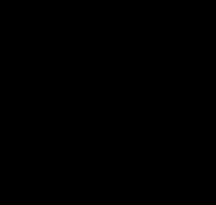
\includegraphics[scale=1.0]{./gw/greenpoles.pdf}
\end{center}
\caption{\small \label{fig:greenpoles} Pole structure 
of the Green's function. 
The occupied electronic states are
slightly above the real frequency axis and below the chemical 
potential $\mu$, the unoccupied states are located above the Fermi
level and slightly below the real axis. The poles of the Green's 
function correspond to the addition/removal energies 
in the system. This example is for a system with a discrete series of 
excitations and an energy gap between occupied and unoccupied states
of $E_{g}$.}
\end{figure}
%
To demonstrate this it is necessary to Fourier transform the Green's from the time
domain to the frequency domain. This can be accomplished by 
rewriting the field operators in the Heisenberg representation:
%
\begin{equation}
\label{eq:heisenop}
\cfield(\r,t) = e^{i\hat{H}t}\cfield(\r) e^{-i\hat{H}t}.
\end{equation}
%
We then introduce a complete set of states which describe all the possible 
intermediate excitations of the system to $N'$ particles 
and their $s$ excited states,~$|N',s\ket$:
%
\begin{equation}
\label{eq:compstates}
\sum_{s}|N', s\ket \bra N',s| = \I,
\end{equation}
%
where $\I$ is the identity matrix.
We also note that:
%
\begin{equation}
H|N,s\ket = E^{s}_{N}|N,s\ket.
\end{equation}
%
%
If one inserts Eqs. \ref{eq:heisenop} and \ref{eq:compstates} into Eq.~\ref{eq:green} it is possible 
to write the Green's function in the time domain as:
%
\begin{align}
\label{eq:grtimedom}
G(\r,t,\rp,t') & = & \sum_{s} -i\Theta(t-t') e^{i(E^{0}_{N} - E_{N'}^{s})(t-t')}\bra N|\field(\r)|N',s\ket\bra N',s|\cfield(\r')|N\ket \nonumber \\
	  &+ & \sum_{s} i\Theta(t'-t) e^{-i(E_{N}^{0} - E^{s}_{N'})(t-t')}\bra N|\cfield(\r') |N',s\ket \bra N',s|\field(\r)| N \ket.
\end{align}
%
Now Eq.~\ref{eq:grtimedom} gives the Green's function in the time domain and the arguments depend 
only on differences in time $t-t'$. By introducing the time variable $\tau = t-t'$ it is 
straightforward to define a Fourier transform:
%
\begin{equation}
G(\r,\r';\omega) = \frac{1}{2\pi} \int_{-\infty}^{\infty} G(\r,\r,\tau) e^{i\omega\tau} d\tau,
\end{equation}
%
and represent the Green's function in the frequency domain:
%
\begin{eqnarray}
\label{eq:greenfreq}
G(\r,\rp;\omega) & = &\sum_{s} \frac{\bra N|\field(\r) |N',s\ket \bra N',s|\cfield(\r')| N \ket}{\omega - (E^{s}_{N'} - E^{0}_{N}) + i\delta} \nonumber \\
	  		   & - & \sum_{s}\frac{\bra N|\cfield(\r') |N',s\ket \bra N',s|\field(\r)| N \ket}{\omega + (E^{s}_{N'} - E^{0}_{N}) - i\delta}.
\end{eqnarray}
%
The infinitesimal factors of $i\delta$ ensure that the Fourier 
transform converges at infinite time arguments.
The presence of the field operators implies that the only 
non-zero contributions to Eq.~\ref{eq:greenfreq} are between 
the ground and excited states of the $N'=N+1$ and the $N'=N-1$ systems. 
Therefore it is convenient to make the follow substitution~\cite{inkson}:
%
\begin{equation}
(E^{s}_{N+1} - E^{0}_{N}) = \epsilon^{s}_{N+1},
\end{equation}
%
with a similar expression for the $N-1$ system. The variable $\epsilon^{s}_{N\pm1}$ 
is the energy difference of an excited state in the $N\pm1$ many body system and 
the ground state of the $N\pm1$ system. 
This leads us to:
%
\begin{eqnarray}
\label{eq:greenpoles}
G(\r,\rp;\omega) = \sum_{s} \frac{\bra N|\field(\r) |N+1,s\ket \bra N+1,s|\cfield(\r')| N \ket}{\omega - \epsilon^{s}_{N+1} + i\delta} \nonumber \\
			 		-\sum_{s} \frac{\bra N|\cfield(\r')|N-1,s\ket \bra N-1,s|\field(\r)| N \ket}{\omega + \epsilon^{s}_{N-1} - i\delta}.
\end{eqnarray}
%
The poles of Eq.~\ref{eq:greenpoles} are represented schematically in Fig.~\ref{fig:greenpoles} 
and correspond to the energies of the excitations from $N$ to $N\pm1$ electrons 
in an interacting many body system. Having discussed the pole structure of 
the Green's function we now proceed to define the equation of motion.

\section{Green's function methods}
\noindent
Lars Hedin first developed the $GW$ approximation with
his publication ``New Method for Calculating the One-Particle Green's Function
with Application to the Electron-Gas Problem.''~\cite{hedin65}. In this work Hedin developed a
self-consistent system of equations for including all the interaction effects
in a many electron system. Hedin describes the
connection between his work and the development of Green's
functions methods by Schwinger in Ref.~\cite{schwinger51} 
working in the field of quantum electrodynamics.
An early review of the applications of Green's function methods and
Feynman diagrams to the many electron problem was given in Ref.~\cite{pratt63}. The procedure
has been extensively studied in the 
intervening thirty years and Refs.~\cite{aulbur00, aryasetgunnarsson98, onida02}
provide a review of the contemporary state of the field.
%
\subsection{Equation of motion}
\noindent
To derive the equation of motion for the Green's 
function we need the time derivative of Eq.~\ref{eq:green}. 
This derivative in turn requires working out the time 
dependence of the field operators appearing in Eq.~\ref{eq:green}:
%
\begin{equation}
\frac{\partial \field(\r,t)}{\partial t} = i[\hat{H},\field(\r,t)].
\end{equation}
%
The time dependence of the field operator is determined by the 
commutator between the Hamiltonian and the field operator.
%
The general Hamiltonian we will consider can be separated into two parts:
%
\begin{equation}
\H =  \H_{0} + v(\r,\r')\delta(t-t'),
\end{equation}
%
where the $\H_{0}$ term describes the kinetic energy of the electron and the interaction of the 
electron with an ionic lattice. 
The $v(\r,\r')\delta(t-t')$ term represents the inter-electron Coulomb repulsion.
We differentiate Eq.~\ref{eq:green} with respect to time to arrive at the following result:
%
\begin{align}
\label{eq:greqmotn}
\left[i\frac{\partial}{\partial t} - \H_{0}\right]G(\r,\r',t,t') +  & &  \nonumber \\
i\int v(\r,\r'')\bra N| T[\cfield(\r'',t)\field(\r'',t)\field(\r,t)\cfield(\rp,t')] |N \ket d\r'' & = & \delta(\r-\rp)\delta(t-t').
\end{align}
%
The right hand side of Eq.~\ref{eq:greqmotn} comes immediately from 
the fact that $\frac{\partial}{\partial t}\Theta(t-t') =\delta(t-t')$, 
and the anti-commutator identity for fermionic field operators. 
%
The commutator for the single particle operator, $\H_{0}$, and the 
field operator can be separated directly. 
The final term under the integral sign results from the commutator
involving the field operators and the Coulomb interaction.

The number of indices that we require to keep track of everything when 
describing multi-particle propagators, and, in the next section, 
when taking functional derivatives, can be very large. 
Therefore, in order to proceed, we will employ the compressed notation for space, 
time, and spin: $1 = (\r,t,\sigma)$, $2=(\r',t',\sigma')$, and so on.

The quantity under the integral sign in Eq.~\ref{eq:greqmotn} is a two particle Green's function:
%
\begin{equation}
\label{eq:2pgreenfxn}
G_{2}(1,2,3,4) = \frac{1}{i^{2}} \bra N|T[\cfield(4)\cfield(3)\field(2)\field(1)]|N\ket.
\end{equation}
%
Eq.~\ref{eq:greqmotn} expresses the single particle Green's function now defined 
implicitly in terms of the two particle Green's function. The two particles Green's function is 
defined in terms of  four field operators. The equation of motion for the two particle Green's 
function would then involve terms with an increasing number of field operators due to the coupling 
via the Coulomb interaction.
This is the heart of the many body problem: an infinite expansion of interaction terms,
all of comparable magnitude, due to the strength of the Coulomb coupling.

When trying to solve equations of the form Eq.~\ref{eq:greqmotn} it is convenient to 
replace the function appearing under the integral sign with a new function,
termed a kernel, and then attempt to solve the system of equations in terms of this kernel.
In order to solve Eq.~\ref{eq:greqmotn} and derive the $GW$ approximation,
we will introduce three new quantities: $\Sigma$, $P$ and $\Gamma$.
Respectively these are named the self-energy, the polarization propagator, and the vertex function.
At this stage we introduce the self-energy $\Sigma$, by rewriting the integrand in Eq.~\ref{eq:greqmotn} as:
%
\begin{equation}
\label{eq:greqmsig}
\left[i\frac{\partial}{\partial t} - \H_{0}\right]G(\r,\r',t,t') - \int \Sigma(\r,\r'',t,t'')G(\r'',\rp,t'',t')d\r''dt'' =  \delta(\r-\rp)\delta(t-t').
\end{equation}
%
The equation now has the shape that we discussed in Sec.~\ref{sec:thelda} when discussing
the generalized Kohn-Sham exchange correlation potential. The Green's 
function evolves under the single particle
interactions included in $\H_{0}$ and according to some non-local, energy dependent potential, $\Sigma$.
What remains to be done is to show how we can calculate $\Sigma$ efficiently, and remove the 
implicit definition of the Green's function in terms of multi-particle propagators.

\subsection{Functional derivative of the Green's function}
\noindent
Eq.~\ref{eq:greqmotn} defines the equation of motion for the one particle Green's
function by making reference to the two particle Green's function.
In the following we will rewrite the equation of motion so that it is entirely defined in
terms of the single particle Green's function. This can be
accomplished by relating the single particle Green's function to the two particle Green's
function via a functional derivative.

To derive Hedin's equation we make some formal modifications. The following derivation follows closely
that presented in Appendix A of Ref.~\cite{hedin65}, the review article of \cite{strinati88} 
and the textbook of Inkson \cite{inkson}. A few important functional identities 
are reproduced in Appendix~\ref{app:funcdiv}. These are required to manipulate the equations 
and obtain their final closed form.

First Eq.~\ref{eq:greqmotn} is rewritten to include a perturbing potential $\phi(1)$:\footnote{For our
purposes a local scalar potential $\phi(1)$ is sufficient to derive the $GW$ approximation. More general 
perturbations, e.g. coupling to non-local vector potentials, are developed in Ref.~\cite{strinati88}.}
%
\begin{align}
\label{eq:greqmotn2}
\left[i\frac{\partial}{\partial t} - \H_{0} - \phi(1)\right]G(1,2) +& \nonumber \\
i\int v(1,3)\delta(t_{3}-t_{1})\bra N| T[\cfield(3)\field(3)\field(1)\cfield(2)] |N \ket d3 &= \delta(1,2).
\end{align}
%
The perturbing potential will be set to zero at the end of the derivation.

Eq.~\ref{eq:greqmotn2} allows us to separate motion generated by the original Hamiltonian, 
which is composed of the single electron and electron-electron
interaction terms, from the time development due to the perturbation $\phi(1)$. The perturbing potential 
allows us to define the functional derivative of the system's Green's
function, and hence relate the propagation of a single particle to the propagation of multiple particles. 
The introduction of $\phi(1)$ allows us to generate an infinite series of terms 
describing the electron-electron interactions in terms of functional derivatives.

Eq.~\ref{eq:greqmotn2} is rewritten so that the field operators refer to the ground-state field
operators, denoted $\field_{0}$, and their time development due to $\phi(1)$ is made explicit:
%
\begin{equation}
\label{eq:intergr}
G(1,2) =  \frac{\bra N|\hat{T}[\hat{S}\field_{0}(1)\cfield_{0}(2)]|N\ket}{\bra N| \hat{S} |N\ket}.
\end{equation}
%
The $\hat{S}$ operator propagates the ground-state field operators according to:
%
\begin{equation}
\hat{S} = T\rm{exp}\left[-i\int_{t_{1}}^{t_{2}} \phi(2)\field_{0}(2)\cfield_{0}(2)d{2}\right].
\end{equation}
%
This separation ensures the time development of the field operators due to $\phi$ is made explicit
and the field operators have no implicit dependence on the perturbation. In this way the field 
operators reflect only the dynamics of the underlying electron system interacting via the Coulomb interaction.

By functional differentiation of Eq.~\ref{eq:intergr} with respect to the perturbing potential $\phi$ 
the two particle Green's function can be written:
%
\begin{equation}
\label{eq:funcdifgr}
G(1,3,2,3^{+}) = G(1,2)G(3,3^{+}) - \frac{\delta G(1,2)}{\delta \phi(3)}.
\end{equation}
%
To arrive at Eq.~\ref{eq:funcdifgr} we used the quotient rule as it applies to functional derivatives, 
and that the variation in $S$ is:   
%
\begin{equation}
\frac{\delta \hat{S}}{\delta\phi(3)} = i \hat{S} \field(3)\cfield(3).
\end{equation}
%
We can now use Eq.~\ref{eq:funcdifgr} to replace the two particle propagator in Eq.~\ref{eq:greqmotn}:
%
\begin{align}
\label{eq:greqmwfd}
\left[i\frac{\partial}{\partial t}-\H_{0}(1)-V(1)\right]G(1,2) &
	-i\int v(1,3)\frac{\delta G(1,2)}{\phi(3)}d3 &=\delta(1,2),
\end{align}
%
where: 
%
\begin{equation}
V(1) = \phi(1) - i\int v(1,3) G(3,3^{+})d3.
\end{equation}
%
Eq.~\ref{eq:greqmwfd} has now separated into two terms. The first term
contains the single electron components
of the Hamiltonian, the perturbing potential, and what can now be
identified as the Hartree potential, i.e. the mean field
felt by an electron due to the classical potential generated from the electron cloud 
discussed in Section~\ref{sec:hohnkohn}. The connection can be seen directly 
by noting that the quantity $G(3,3^{+})$ is just the electronic density. 
\footnote{It is important to see this connection: the diagonal elements 
of the Green's function are just the electron density. 
The superscript $+$ is added to avoid problems
with the definition of the step function in the time 
domain when $(t-t')=0$.}

The second term contains the \emph{bare} Coulomb interaction 
multiplied by the functional derivative of the 
one particle Green's function. Upon comparison of 
Eq.~\ref{eq:greqmwfd} with Eq.~\ref{eq:greqmsig} we can 
rearrange terms by observing:
%
\begin{equation}
\int \Sigma(1,3)G(3,2)d3 = -i\int v(1,3) \frac{\delta G(1,2)}{\delta \phi(3)}d3,
\end{equation}
%
or by isolating the self-energy $\Sigma$ as: %(where we have used app. 1 Eq.~\ref{eq:expansionrule}):
%
\begin{equation}
\label{eq:sigma}
\Sigma(1,2) = i \int v(1,4) G(1,3) \frac{\delta G^{-1}(4,2)}{\delta\phi(4)}d3d4.
\end{equation}
%
We now retrieve the equation of motion for the Green's function 
as it appeared in Eq.~\ref{eq:greqmsig} as:
%
\begin{equation}
\label{eq:greqmsig2}
\left[i\frac{\partial}{\partial t} - \H_{0}(1) - V(1)\right]G(1,2) - i\int \Sigma(1,3)G(3,2)d3 = \delta(1,2).
\end{equation}
%
One could formally solve this equation as it stands using an iterative method, 
however it is worth noting that the resulting expansion of the self-energy $\Sigma$ 
would contain increasing powers of the bare Coulomb interaction $v$. 
It is unlikely that the resulting series will converge particularly 
quickly, if it converges at all. 
%
Therefore it is necessary to expand $\Sigma$ in a closed form without making 
reference to the perturbing potential $\phi$. In doing so the equations are rearranged so that
the bare Coulomb interaction is modified and the electrons experience 
an effective screened Coulomb interaction. In a classical picture the electrons will interact
via a Coulomb interaction screened by the system's dielectric function. 
This will be done in the next two sections.
%
\section{Hedin's equations}
\subsection{Dielectric function}
\label{sec:dielecfun}
\noindent
At this point it is useful to introduce the following functional relationships 
which define the dielectric function in a many-body system.
We will switch back to labeling time and space coordinates as $\r,t$ 
here for ease of reference Section~\ref{sec:nscfstern}. 

The effective potential acting on the electrons is:
%
\begin{equation}
\label{eq:internalpot}
V(\r,t) = \phi(\r,t) - i\int v(\r,\r') G(\r',\r',t,t^{+}) d\r',
\end{equation}
%
where $iG(\r',\r',t,t^{+})$ is the single particle density $n(\r')$.
%
We now define the inverse dielectric function to be the self-consistent variation 
of this effective potential with respect to the external perturbing potential:
%
\begin{equation}
\label{eq:invepsvphi}
\inveps(\r,t,\r',t') = \frac{\delta V(\r,t)}{\delta\phi(\r',t')}.
\end{equation}
%
Upon inserting Eq.~\ref{eq:internalpot} into Eq.~\ref{eq:invepsvphi} we arrive at:
%
\begin{equation}
\label{eq:simpphys}
\inveps(\r,t,\r',t') = \delta(\r-\r')\delta(t-t') + \int v(\r,\r'') \frac{\delta n(\r'',t)}{\delta\phi(\rp,t')}d\r''.
\end{equation}
%
Eq.~\ref{eq:simpphys} has a simple physical interpretation. The inverse dielectric function 
encodes the self-consistent variation in the charge density 
with respect to a variation in the potential $\phi$.
This rearrangement of charge means that the bare Coulomb interaction
 between two points is altered by the induced screening in
the interacting medium. This altered Coulomb interaction is the 
screened Coulomb interaction, and can be defined 
in terms of the inverse dielectric function as:
%
\begin{equation}
\label{eq:scrncoul}
W(\r,t,\r',t') = \int v(\r,\r'')\delta(t-t'') \frac{\delta V(\r',t')}{\delta \phi(\r'',t'')} dr''dt''.
\end{equation}
%
The screened Coulomb interaction can also be written as an integral equation: 
%
\begin{equation}
\label{eq:dysw}
W(\r,t,\r',t') =  v(\r,\r') + \int d\r''' v(\r,\r''')\int P(\r''',t,\r'',t'') W(\r'',t'',\r',t')dt''d\r''.
\end{equation}
%
where the polarizability, $P$, has been introduced:
%
\begin{equation}
P(\r,\r',t,t') = \frac{\delta n(\r',t')}{\delta V(\r,t)}.
\end{equation}
%
Alternatively we can introduce the dielectric function in its non-inverted form as:
%
\begin{equation}
\label{eq:epschap2}
\epsilon(\r,t,\rp,t') = \delta(\r-\r')\delta(t-t') - \int v(\r,\r'') P(\r'',t'',\r',t') \delta(t-t'') d\r''dt''.
\end{equation}

\subsection{Hedin's equations}
\noindent
While the Coulomb repulsion between electrons remains the bare Coulomb interaction, 
the dielectric function provides a route to interpreting 
an auxiliary system of electrons interacting via a \emph{screened} Coulomb interaction.

In order to include this screening implicitly in the definition of the self-energy, we 
go back to the definition of $\Sigma$ in Eq.~\ref{eq:sigma}. We now use the chain 
rule to take the functional derivative of $G$ with 
respect to the total potential $V$ rather than the perturbing potential $\phi$:
%
\begin{equation}
\label{eq:funcdifsig}
\Sigma(1,2) =  i\int v(1,4) G(1,3)\frac{\delta G^{-1}(3,2)}{\delta V(5)}\frac{\delta V(5)}{\delta\phi(4)}d3d4d5.
\end{equation}
%
By comparison of Eqs. \ref{eq:invepsvphi}, \ref{eq:scrncoul}, and \ref{eq:funcdifsig} we can combine
the inverse dielectric function and the bare Coulomb interaction into the screened Coulomb interaction $W$:
%
\begin{equation}
\Sigma(1,2) =  i\int W(1,4)G(1,3)\frac{\delta G^{-1}(3,2)}{\delta V(4)}d3d4.
\end{equation}
%
The final piece of notation to be introduced is the vertex function. This is defined as the variation 
of the inverse Green's function with respect to the potential $V$:
%
\begin{equation}
\label{eq:vertex}
\Gamma(1,2;3) = \frac{\delta G^{-1}(1,2)}{\delta V(3)}.
\end{equation}
%
Having obtained the expression for the vertex function in Eq.~\ref{eq:vertex} we
can write all of Hedin's equations in a closed form.
We summarize Hedin's equations describing the interacting Green's function,
the screened Coulomb interaction, the polarizability, and the vertex function of the system:
%
\begin{align}
\label{eq:hedinsig}
&\Sigma(1,2)   = i\int W(1^{+},4)G(1,3)\Gamma(3,2;4)d4d3 &   \\
\label{eq:hedinw}
&W(1,2)        =  \int \inveps(1,3)v(3,2) d3 &               \\
\label{eq:hedineps}
&\epsilon(1,2) =  \delta(1,2) - \int v(1,3)P(3,2)d3 &        \\
\label{eq:hedinpol}
&P(1,2)        = -i\int G(1,3)\Gamma(3,4;2) G(4,1^{+})d4d3 & \\
\label{eq:hedinvert}
&\Gamma(1,2;3) = \delta(1,2)\delta(1,3) + \int \frac{\delta\Sigma(1,2)}{\delta G(4,5)}G(4,6)G(7,5) \Gamma(6,7;3)d4d5d6d7 & 
\end{align}

In summary, we started from the equation of motion. Then a relationship between
the two particle Green's function and the one particle Green's function was found.
This relationship takes the form of a functional derivative of the one particle Green's function with
respect to a perturbing potential. When everythin is written in terms 
of the one particle Green's function we have obtained a set of equations 
that need to be solved self-consistently. 
These are known as Hedin's equations. When solved iteratively these 
equations incorporate all the many body effects of a many-electron system.

\section{$G_0W_0$ self-energy and corrections to LDA eigenvalues}
\noindent
In the first section of this chapter we have discussed the
procedure for constructing the $G_0W_0$ self-energy operator.
We have also discussed some of the considerations required when
performing DFT calculations within a planewaves basis set.
It remains to show how the $G_0W_0$ self-energy can be
used to connect the eigenvalues obtained from a DFT calculation.

We proceed as in Ref.~\cite{HL86} by assuming the $G_0W_0$
self-energy can be treated as a perturbation to the
DFT Kohn-Sham exchange and correlation potential.

In Chapter~\ref{chap:dftgw} we discussed the quasiparticle equation:
%
\begin{equation}
\label{eq:qpeq2}
\left[-\frac{1}{2}\nabla^{2} + \hat{V}^{\rm{ion}} + \hat{V}^{\rm{H}}\right]\phi_{n\k}(\r) + \int{d}\r' \Sigma(\r,\r';E_{n\k})\phi_{n\k}(\r')=E_{n\k}\phi_{n\k}(\r).
\end{equation}
%
By adding and subtracting $V_{xc}(\r)\psi_{n\k}(\r)$ one obtains:
%
\begin{equation}
(-\frac{1}{2}\nabla^{2} + \hat{V}^{\rm{ion}} + \hat{V}^{\rm{H}} + \hat{V}^{\rm{xc}})\phi_{n\k}(\r) + \int{d}\r' \left[\Sigma(\r,\r';E_{n\k})-\hat{V}^{\rm{xc}}(\r')\delta(\r,\r')\right]\phi_{n\k}(\r') = E_{n\k}\phi_{n\k}(\r).
\end{equation}
%
If we treat $\Sigma-V^{\rm{xc}}$ as a perturbation we can express $E_{n\k}$
in terms of the Kohn-Sham eigenvalues $\epsilon^{\rm{LDA}}_{n\k}$ using 
first order perturbation theory:
%
\begin{equation}
\label{eq:QPenergy}
E_{n\k}^{\rm{QP}} = \epsilon_{n\k}^{\rm{LDA}} + \bra n\k| \Sigma(E_{n\k}^{\rm{QP}}) - \hat{V}^{\rm{xc}}|n\k\ket.
\end{equation}
%
Following Ref.~\cite{HL86} we expand the self-energy operator to first order around the LDA eigenvalue:
%
\begin{equation}
\label{eq:sigmafirst}
\Sigma( E_{nk}^{\rm{QP}} ) = \Sigma(\epsilon_{nk}^{\rm{LDA}}) + \frac{\partial\Sigma(\omega)}{\partial \omega}\bigg|_{\omega = \epsilon_{n\k}^{\rm{LDA}}}(E_{n\k}^{\rm{QP}} - \epsilon_{n\k}^{\rm{LDA}}). 
\end{equation}
%
The quasiparticle energy can than be obtained by substituting Eq.~\ref{eq:sigmafirst} into Eq.~\ref{eq:QPenergy}:
%
\begin{equation}
\label{eq:QPfirst}
E_{n\k}^{\rm{QP}} = \epsilon_{n\k}^{\rm{LDA}} + \left(1-\frac{\partial\Sigma(\omega)}{\partial \omega}\bigg|_{\omega=\epsilon_{n\k}^{\rm{LDA}}}\right)^{-1}(E_{n\k}^{\rm{QP}} - \epsilon_{n\k}^{\rm{LDA}}). 
\end{equation}
%
The quasiparticle renormalization value $Z$ is defined by:
%
\begin{equation}
Z_{n\k} =  \left[1-\frac{\partial\Sigma(\omega)}{\partial \omega}\bigg|_{\omega = \epsilon_{n\k}^{\rm{LDA}}}\right]^{-1}.
\end{equation}
%
In summary, we find the expression for the $G_{0}W_{0}$ perturbative correction to the LDA eigenvalues is:
%
\begin{equation}
\label{eq:qpcorrpert}
E^{\rm{QP}}_{n\k} =  \epsilon^{\rm{LDA}}_{n\k} + Z_{n\k}\bra n\k|\Sigma(\epsilon^{\rm{LDA}}_{n\k})-V^{xc}_{n\k}| n\k\ket.
\end{equation}
%

\section{The Spectral function}
\subsection{The $GW$ spectral function}
\label{sec:spec}
\noindent
In this section we introduce the spectral function. For simplicity we will contract the
Bl\"och notation $n\k$ to a single index $n$, and then reintroduce the full Bl\"och notation when
we arrive at the final expression for the spectral function.

Given a set of single particle eigenvectors $\phi_{m}(\r)$ we can take matrix elements of the
single particle states with the Green's function and self-energy:
%
\begin{eqnarray}
G_{mn}(\omega)       = \int \int \phi_{m}^{\star}(\r) G(\r,\r';\omega) \phi_{n}(\r')  d\r d\r', \\
\Sigma_{mn}(\omega)  = \int \int \phi_{m}^{\star}(\r) \Sigma(\r,\r';\omega) \phi_{n}(\r') d\r d\r'.
\end{eqnarray}
%
We can employ the same notation for matrix elements with $V^{\rm{xc}}(\r)$,
and the Kohn-Sham Hamiltonian $\hat{H}^{\rm{KS}}$.
%
In matrix notation the Dyson equation \cite{inkson} can be written:
%
\begin{equation}
\label{eq:matdys}
G^{-1} = G_{0}^{-1} - [\Sigma(\omega) - V_{\rm{xc}}].
\end{equation}
%
Eq. \ref{eq:matdys} gives the expression for interacting Green's function.
We note that the exchange and correlation potential of the ground state
calculation is subtracted from the final self-energy. If the Green's function is diagonal
in the state indices we can invert each element of the matrix and write:
%
\begin{equation}
G_{nn}(\omega) = \frac{1}{\omega -\epsilon^{\rm{KS}}_{n}+{\rm Re}\Sigma_{nn}(\omega)-V^{\rm{xc}}_{nn}+{\rm Im}\Sigma_{nn}(\omega)}.
\end{equation}
%
In the case where the non-diagonal elements cannot be ignored,
a full matrix inversion would be required to construct the Green's function:
%
\begin{equation}
G_{mn}(\omega) = [\omega \delta_{mn} - \epsilon^{\rm{KS}}_{mn}\delta_{mn} + {\rm Re}\Sigma_{mn}(\omega) - V^{\rm{xc}}_{nn} + {\rm Im}\Sigma_{mn}(\omega)]^{-1}.
\end{equation}

We can employ the same notation for matrix elements with $V^{\rm{xc}}(\r)$,
and the Kohn-Sham Hamiltonian $\hat{H}^{\rm{KS}}$.
%
In matrix notation the Dyson equation \cite{inkson} can be written:
%
\begin{equation}
\label{eq:matdys}
G^{-1} = G_{0}^{-1} - [\Sigma(\omega) - V_{\rm{xc}}].
\end{equation}
%
Eq. \ref{eq:matdys} gives the expression for interacting Green's function.
We note that the exchange and correlation potential of the ground state
calculation is subtracted from the final self-energy. If the Green's function is diagonal
in the state indices we can invert each element of the matrix and write:
%
\begin{equation}
G_{nn}(\omega) = \frac{1}{\omega -\epsilon^{\rm{KS}}_{n}+{\rm Re}\Sigma_{nn}(\omega)-V^{\rm{xc}}_{nn}+{\rm Im}\Sigma_{nn}(\omega)}.
\end{equation}
%
In the case where the non-diagonal elements cannot be ignored,
a full matrix inversion would be required to construct the Green's function:
%
\begin{equation}
G_{mn}(\omega) = [\omega \delta_{mn} - \epsilon^{\rm{KS}}_{mn}\delta_{mn} + {\rm Re}\Sigma_{mn}(\omega) - V^{\rm{xc}}_{nn} + {\rm Im}\Sigma_{mn}(\omega)]^{-1}.
\end{equation}

At this stage we introduce the spectral function by defining it in terms of the Green's function:
%
\begin{equation}
A_{mn}(\omega) = {\rm Im} |G_{mn}(\omega)|.
\end{equation}
%
Reintroducing the Bloch notation we can write the full spectral function
for the diagonal Green's function:
%
\begin{equation}
\label{eq:aspec}
A_\k(\omega) = \frac{1}{\pi}\sum_{n} \frac{|{\rm Im}\Sigma_{n\k}(\omega)|}
{[\omega- \epsilon_{n\k}-({\rm Re}\Sigma_{n\k}(\omega) -V^{\rm{xc}}_{n\k})]^{2} + \left[{\rm Im}\Sigma_{n\k}(\omega)\right]^{2}}.
\end{equation}

The spectral function helps clarify the quasiparticle picture. Eq.~\ref{eq:aspec} is strongly
peaked when the frequency $\omega$ sweeps through the renormalized
eigenvalue $\epsilon_{n\k} + {\rm Re}(\Sigma_{n\k}(\omega) - V^{\rm{xc}}_{n\k}) $. Given
the frequency dependence of $\Sigma$ additional zeros in the real part of the
denominator of Eq. \ref{eq:aspec} are possible. These can correspond to the
appearance of new excitations which are not present in the non-interacting system. Finally
the imaginary part of the self-energy introduces a broadening of the the quasiparticle peak
and is associated with lifetime effects.

\subsection{Contact with experiment}
\noindent
Angle Resolved Photoemission Spectroscopy (ARPES) is a very useful
probe for investigating the electronic structure of materials~\cite{damascelli04}.
%Incident radiation on a sample can excite electrons via the photoelectric effect. 
%These excited electrons can then propagate to a detector where their energy and momentum 
%is measured. Given the momentum and energy of the impinging light source it is 
%possible to determine the initial electronic state the captured electron occupied 
%in the material. 
%
The intensity of the electrons captured at the experimental detector, $I_{\k}(\omega)$,
can be expressed in terms of the quasiparticle spectral function~\cite{damascelli04}:
%
\begin{equation}
\label{eq:photoemission}
I_{\k}(\omega) = I_{0}(\k,\nu)f(\omega)A_{\k}(\omega),
\end{equation}
%
Where $\nu$ is the frequency of the incident radiation and $f(\omega)$ is the Fermi-Dirac distribution.
The factor $I_{0}(\k,\nu)$ includes matrix element effects, i.e.
the strength of the coupling of the initial and final electron states via
the electromagnetic probe, the effect of surfaces, and 
inelastic scattering in the sample~\cite{damascelli04}.

\subsection{Bardyszewski-Hedin theory of photoemission}
\noindent
A comprehensive analysis of the connection between the spectral function
and photoemission data is given by Bardyszewski and Hedin in Ref.~\cite{bardy85}.
Their formulation begins by relating the photocurrent, $J$, i.e. the number
of electrons ejected from the sample, per unit solid angle and energy
to the intensity, $I$, measured at the detector:
%
\begin{equation}
\frac{\partial^{2}J}{\partial \Omega \partial \epsilon_{\k}} \sim I.
\end{equation}
%
The standard definition for the intensity is then given in Refs.~\cite{goldberger64, almbladh83}:
%
\begin{equation}
\label{eq:intens}
I = \sum_{s}|\bra \k,N-1,s|\hat{\Delta}|N\ket|^{2}\delta(\epsilon_{\k}-\epsilon_{s}-\omega).
\end{equation}
%
The $|\k,N-1,s\ket$ state is a product state of the photoelectron with wave vector
$\k$ and the $|N-1, s\ket$ many electron wavefunction described in Eq. \ref{eq:compstates}.
The frequency of the incoming radiation is $\omega$. The $\hat{\Delta}$
operator is the electric dipole operator.

Eq.~\ref{eq:intens} explicitly couples many-body states via the dipole operator.
The intrinsic contribution of a particular photoelectron $\tilde{\phi}_{\k}$, to the measured photocurrent
can now be written in terms of the one-electron spectral
function discussed in Section~\ref{sec:spec}~\cite{bardy85}:
%
\begin{equation}
\label{eq:barhed}
I(\k,\omega)=\int \tilde{\phi}^{\star}_{\k}(\r)\hat{\Delta}(\r)A(\r,\r';\epsilon_\k-\omega)\hat{\Delta}(\r')\tilde{\phi}_{\k}(\r')d\r d\r'.
\end{equation}
%
If we assume the spectral function is diagonal in $\r$, $\r'$, and exploit the matrix
notation for the spectral function from the previous section we arrive at the expression:
%
\begin{equation}
I(\k,\omega) \approx \sum_{n} |\bra\tilde{\phi}_{\k}|\hat{\Delta}|\phi_{n}\ket|^{2} A_{nn}(\epsilon_{\k}-\epsilon_{n}-\omega).
\end{equation}
%
The photoelectron will not generally travel unimpeded to the detector. 
Along the way the photoelectron can scatter off of phonons, plasmons, 
or other particle-hole excitations.
Ref. \cite{bardy85} provides a detailed derivation of the 
expressions reported here for the intrinsic intensity
of the photocurrent and the possible types of quasiparticle 
excitations in an interacting system.
These results are mentioned here because they provide a direct 
connection between experimental probes and the mathematical 
formalism of the $GW$ approximation.

\section{Alternative Functionals and Tight Binding}
Armed with the local density approximation, a computer, 
and the comfort of a well defined variational principle
means computational material scientists are in a position 
to go out and do a significant amound of damage. In 
this section it is useful to look at a few different functional
forms.

The first constraint we have is $\int\rho(\r)d^{3}\r = N$ incorporating this
constraing using a Lagrange multiplier technique with the fact that we want
to find a variational minimum for the energy we can write:
%
\begin{equation}
\frac{\delta}{\delta \rho} \left[E[\rho] - \mu(\int \rho(\r)d\r - N)\right] = 0,
\end{equation}
%
which leads to:
%
\begin{equation}
\frac{\delta E[\rho]}{\delta \rho}= \mu.
\end{equation}

\section{Purely Functional Forms}
Finnis' textbook gives a comprehensive discussion of functionals,
the Hohenberg-Kohn Functional and the Harris-Foulkes functional.
His development is far more thorough than what is discussed here. 
The important connections to make in the present collection
is that we can point out a direct connection between the

\begin{itemize}
\item A direct relation between the second nd order variation in $E_{\rm xc}$ and the dielectric function can be made.
\item We can define the Generalized Harris-Foulkes Functional which will clarify our ideas about optimizing the computed
      electron densities and changing the potentials we are asking the electrons to move in.
\end{itemize}

The first point means we can connect the exchange-correlation functional, 
which is mysterious and foreign, to a dielectric function, which has a pleasing 
classical picture and is familiar.

The second point is essential because it will justify the use of certain 
computational approaches and clarify why, in some cases, a single shot GW
calculation might ``work", and where it might not. The Generalized Harris-Foulkes
and quantify what is meant by an optimum model of our system and allow for the
construction of densities and potentials that reach this optimum position in 
the functional space. 

The text of this section will be kept to a minimum. It should be viewed as a
useful collection of functional definitions all contained in one place. 
The Hohenberg-Kohn-Sham Energy written in its pure functional form,
as a set of non-interacting electrons, expanded to first order, expanded to
second order, and the Harris-Foulkes function are all discussed.

\subsection{HKS}
\begin{equation}
\label{eq:hks}
E^{\rm HKS} = T[\rho] + E_{\rm H}[\rho] + E_{\rm xc}[\rho] + E_{\rm eZ}[\rho] + E_{\rm ZZ}
\end{equation}

Taking the variation of Eq.~\ref{eq:hks} with respect to the density gives:
%
\begin{equation}
\frac{\delta E^{\rm HKS}}{\delta \rho} = \frac{\delta T[\rho]}{\delta \rho} + V_{\rm H}[\r] + V_{\rm xc}[\r] + V_{\rm ext}[\r] = \mu
\end{equation}
%
where $V_{xc} = \frac{\delta E_{xc}[\rho]}{\delta \rho}$.

In the local density approximation:
%
\begin{equation}
E_{\rm xc}[\rho] = \int\epsilon^{xc}[\rho(\r)]\rho(\r)dr
\end{equation}
%
with epsilon taking its value for the homogeneous electron gas at 
every point. As a potential the chain rule needs to be used to obtain:
%
\begin{equation}
\frac{\delta E_{\rm xc}[\rho(\r)]}{\delta \rho(\r)} = \epsilon^{xc}(\r) + \frac{d \epsilon^{xc}[\rho(\r)]}{d\rho}|_{\rho(\r)}\rho(\r)
\end{equation}
%

If the Kohn-Sham trick of introducing a set of non-interacting electrons is used the Energy can be written
%
\begin{equation}
E^{\rm HKS}[\rho] = \sum_{i}f_{i}\bra \psi_{i}|\hat{T} + \hat{V}_{\rm eff}|\psi_{i}\ket - \frac{1}{2}\int\rho V_{\rm H} - \int\rho V_{xc} + E_{xc}[\rho] + E_{ZZ}
\end{equation}

\subsection{Harris Fragments}
Harris's approach \cite{harris85} comes from the perspective of bringing together 
"interacting fragments" \footnote{The idea had been treated in K. Nikulin, Zh. Tekhn. Fiz. XLI, 41 (1971) 
[Sov. Phys. — Techn. Phys. 16, 28 (1971)]; R. G. Gordon and Y. S. Kim, J. Chem. Phys. 56,3122 (1972)
see also Wendel and Martin \cite{wenel79}. }
Two separate fragments for which we can obtain the density are brought together. 
The new effective potential is generated from the sum of the fragment's densities, 
and the single particle eigenvalues are recomputed.

The idea is quite intuitive. We take a slab of one thing $n_{1}(x)$ 
and a slab of another thing $n_{2}(x)$ and form the combined density 
$n_{f}= n_1 + n_2$. From the combined density a new effective potential
is generated:

\begin{equation}
\tilde{V}(x) = V^{\rm H}(x) + \mu^{\rm nf}_{\rm xc}(x) + V^{\rm ion}(x)
\end{equation}

The eigenvalues can then be determined for the effective single particle
potential (which contains the exact configuration of ions). 
The total energy of this combined system is then given:
%
\begin{equation}
E_{R} = \sum_{n}a_{n}\tilde{\epsilon} - \int dx n_{f}(x)[\frac{1}{2}V^{\rm H}(x) + \mu_{nf}^{xc}(x)] + E^{\rm xc}[n_f]+ E^{\rm ion}
\end{equation}
%
Writing 
What has been accomplished? Well it seems a little like the trick of adding
two densities together is too simple to be useful. The usefulness lies in the
fact that when the errors introduced by the approximation 
are proportional to $\delta n(r)^2$ and not linear in the density. 

If a good guess at the density can be found, good in the sense the combined 
density is almost equal to the true self-consistent 
density, $n_{f}(r) \approx n(r)$, we have some 
grounds to think that the computed total energies will be as well
and there is no need to solve the self-consistent problem iteratively.

%The error relative to the HKS functional is given \cite{finnis92}:
%\begin{equation}
%E^{HKS}[n^{sc}]- E^{HF}[n^{in}] = \int [n^{out}(r)-n^{in}(r)]U(r,r')
%\end{equation}

The Harris-Foulkes functional eliminates the need to perform multiple iterations
of a self-consistent loop. The idea has been tried in a few different contexts
\cite{harris85, foulkes87, foulkes89, haydock11}.

\subsection{HFG}
The extremal properties of the functional are discussed in Refs.~\cite{finnis, haydock11}.
Finnis places particular emphasis on the expansion of the HKS function to second order in the
variation of the density:

One finds that if $H^{in} = \hat{T}+V_{ext}+V_{H}^{\rm in}+V_{xc}^{\rm in}$,
the kinetic energy functional can be calculated as:
%
\begin{equation}
T_{s}[\rho] = \sum_{i}\bra i|H^{\rm in}|i\ket - \int\rho V_{eff}
\end{equation}

\begin{equation}
\label{eq:sohks}
E^{(2)}[\rho] = \sum_{i}{\bra \psi_{i}|\hat{H}^{\rm in}|\psi_{i}\ket} + E_{\rm xc}^{\rm in}
-\rho^{\rm in}V_{xc}^{in} - E_{H}^{in} + E_{ZZ} + \frac{1}{2}\int C_{in}(\r,\r')\delta\rho\delta\rho'.
\end{equation}

Eq.~\ref{eq:sohks} can be obtained by introducing a density $\rho = \rho^{\rm in} + \delta\rho$, inserting this into
Eq.~\ref{eq:hks} and expanding the terms. 

The second order variation in the Hartree and exchange correlation terms are encoded in
%
\begin{equation}
C_{\rm in}(\r,\r') = \frac{1}{|\r-\r'|} + \frac{\delta^{2}E_{xc}[\rho]}{\delta rho \delta rho'}
\end{equation}

If one has some knowledge of $C(\r,\r')$ than one is in a position where the self-consistency 
requirement can be eliminated and a set of N eigenfunctions only needs to be determined 
before an estimate of the total energy can be written down immediately.

Eq.~\ref{eq:sohks} is minimized by solving:
%
\begin{equation}
\hat{T} + V_{eff}^{(2)}|n\ket= \epsilon_{n}|n\ket
\end{equation}
%
where $V_{\rm eff}^{(2)}=V^{\rm in}_{\rm eff}(\r) + C_{in}(\r,\r')\delta \rho(\r')d\r'$

%Finally note:
%
%\begin{equation}
%E^{\rm HKS}[\rho = E^{(2)} + \Delta E_{\rm xc}^{\rm in}[\rho
%\end{equation}

\subsection{Generalization of the Harris-Foulke Functional}

The Harris Foulkes functional:
%
\begin{equation}
E^{(1)}_{\rm HF}[\rho] = \sum_{i} \bra i |\hat{H}^{\rm in}|i\ket + E_{\rm xc}^{\rm in} - \int \rho^{\rm in}V^{\rm in}_{\rm xc} - E^{\rm in}_{H} + E_{ZZ}
\end{equation}

is variationally minimal with respect to the wave functions, which is equivalent, to it being variationally minimal
with respect to the output density at fixed $rho^{in}$. So it has two co-ordinates that
we can vary to minimize it. The $V^{in}_{eff}$ is a thisd co=ordinate that can be minimized

The generalized Harris-Foulkes functional can be viewed in these terms:
%
\begin{equation}
E^{HFG}[\rho^{out}, \rho^{in}, V_{eff}] = \sum_{i}f_{i}\epsilon_{i}-\rho^{in}V_{eff}+\rho^{in}V_{ext}+E_{xc}^{in}+E_{H}^{in}+E_{ZZ}
\end{equation}
%
$\rho_{in}$ and $V_{eff}$ can strictly speaking be anything you want them to be. This is where the 
craft comes into materials modelling and really choosing them is only dictated by what you
want to calculate and how accurately you would like to calculate it. 

However the functional is only minimized when $\rho^{in} = \rho^{out}$ and $V_{eff}=V_{in}$.
In Fig.~\ref{fig:hfg} a graphical representation of the co-ordinate of the functional.
%
\begin{figure}
\begin{center}
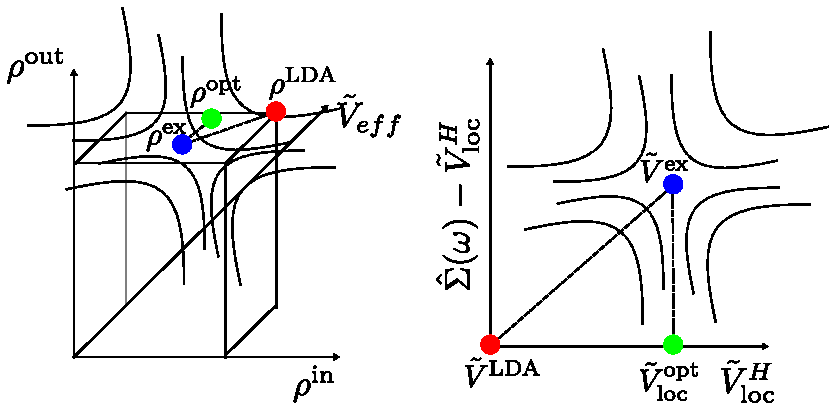
\includegraphics{./GW/HFG_space.pdf}
\caption{Schematic representation of the coordinates for the generalized
Harris-Foulkes functional. Hashed lines represent contours drawn to indicate
a saddle point. The left panel gives stationary points in the co-ordinate space
for different functionals. The blue dot indicates the stationary point for the
LDA Kohn-Sham functional with the exact density $\rho^{ex}$, 
and exact Kohn-Sham energy functional. The green dot gives a stationary point
for a hypothetical "optimal functional". The red dot is a stationary point
for the Kohn-Sham Functional using the local density approximation. The sense in which it is optimal 
is discussed in the text and in Chap.~\ref{chap:manybodyrec}. The
right panel divides the space of effective potentials into a coordinate 
composed of only local Hermitian potentials and an orthogonal co-ordinate 
of non-Hermitian non-local potentials. This is in the spirit of Ref.~\cite{sohrab10}. 
The figure demonstrates how one can approach an optimal
potential which minimizes the distance to the true functional 
while retaining desirable computational properties like being Hermitian and local
or allowing us to avoid multiple iterations to self-consistency.}
\end{center}
\end{figure}
%
The blue dot corresponds to $\rho^{\rm ex}$, and $V^{\rm ex}_{\rm eff}$. The red dot
represents the stationary point for the HKS functional using the LDA.

The important point is that the energy obtained will differ by quantities of second
order smallness in the guessed density, and the effective potential: i.e., 
$(\rho^{\rm in}-\rho^{\rm ex})^{2}$ and $(V_{\rm eff}^{\rm in}-V_{\rm eff}^{\rm ex})^{2}$.
This means with judicious choices we can obtain accurate results with a feasible
amount of computational work.

Finally, the reader may recall the mystery around the first term 
of Eq.~\ref{tb:force} in Chapter~\ref{chap:invariance}. This term is required to complement
the band energy contribution which we can calculate with the recursion technique. However it is
less obvious what form this potential should take. It is often approximated as a pair potential.

If we re-write the total energy following Finnis:
%
%\begin{equation}
%\end{equation}
%
If $\rho_{in}$ in Eq.~\ref{eq:rewrittenHFG} is the charge density for the sum of spherical atomic 
charges then the interacting ion terms will correspond to pair potentials that are rapidly screened. 
These considerations will be developed further in Chapter~\ref{chap:wannier}.

\section{Conclusion}
\noindent
This chapter introduced the Hohenberg-Kohn theorem. This theorem,
which states the ground-state energy of an interacting electronic system 
is a functional of the ground-state charge density is the basis of all the
subsequent discussion. From that theorem much of the rest follows.

The Kohn-Sham scheme was introduced as providing 
a prescription for obtaining a set of wavefunctions, 
and eigenvalues, to describe the ground-state density of a system. 

The various approximations to the exchange correlation 
functional commonly used in applications of Kohn-Sham DFT like the LDA, LDA+U,
GGA, and hybrid functionals are the work horses of materials modelling. 

%For a given configuration of ionsit is commonplace to send a calculation 
%off to a computing machine and within a few
%minutes, hours, or days (depending on the size of the system) come back to directories 
%full of eigenvalues, charge densities, wavefunctions, and total energies.
%We discussed various schemes for extending DFT, a theory for the ground state,
%to describe excited state properties and give us a better treatment of the exchange
%and correlation in real systems. 
We then discussed an approach based on Green's function methods 
to accurately treat processes involving electron addition and removal
to remedy some of the defects present in the use of the local density approximation
to the exchange correlation functional. 

Along these lines we presented a detailed discussion
of the analytic properties of the Green's function and a full derivation of Hedin's
equations which define the $GW$ approximation. Hopefully now the reason it is called
$GW$ is less mysterious \footnote{If the naming remains mysterious you 
should go back and read that section again.}.

The connection to the tight binding formulation of materials science was motivated
in the final section of the $GW$ discussion by sketching out the type of integrals that would 
have to be computed to form the matrix elements of the Green's function and self-energy
operator. The possibility of exploiting a perturbative approach to including
the exchange and correlation energies systematically was discussed in Section~\ref{sec:gwpert}. 
By mapping these operators on to matrix elements and being selective about 
which experimentally accessible quantities we wish to compute 
it should be possible to streamline the calculations into a more manageable framework. 

The formal transformation from DFT/GW methods to functionals
amenable to being described in terms of local short range interactions 
was begun in the section on the Harris-Foulkes functional.
These idea will be developed further in Chapters~\ref{chap:wannier} and \ref{chap:manybodyrec}.
